\documentclass[../Main.tex]{subfiles}

\definecolor{codegreen}{rgb}{0,0.6,0}
\definecolor{codegray}{rgb}{0.5,0.5,0.5}
\definecolor{codepurple}{rgb}{0.58,0,0.82}
\definecolor{backcolour}{rgb}{0.95,0.95,0.92}

\lstdefinestyle{mystyle}{
    backgroundcolor=\color{backcolour},   
    commentstyle=\color{codegreen},
    keywordstyle=\color{magenta},
    numberstyle=\tiny\color{codegray},
    stringstyle=\color{codepurple},
    basicstyle=\ttfamily\footnotesize,
    breakatwhitespace=false,         
    breaklines=true,                 
    captionpos=b,                    
    keepspaces=true,                 
    numbers=left,                    
    numbersep=5pt,                  
    showspaces=false,                
    showstringspaces=false,
    showtabs=false,                  
    tabsize=2
}


\lstdefinelanguage{JavaScript}{
  keywords={typeof, new, true, false, catch, function, return, null, catch, switch, var, if, in, while, do, else, case, break, assertLogin, await},
  keywordstyle=\color{purple}\bfseries,
  ndkeywords={class, export, boolean, throw, implements, import, this, await},
  ndkeywordstyle=\color{darkgray}\bfseries,
  identifierstyle=\color{black},
  sensitive=false,
  comment=[l]{//},
  morecomment=[s]{/*}{*/},
  commentstyle=\color{codepurple}\ttfamily,
  stringstyle=\color{codepurple}\ttfamily,
  morestring=[b]',
  morestring=[b]"
}

\lstset{style=mystyle}

\begin{document}

    \section{Pruebas de regresión}
    \subsection{Descripción}
    \begin{justify}
    La prueba de regresión es un tipo de prueba que se realiza para verificar que un cambio de código en el software no afecta la funcionalidad existente del producto. Esto es para asegurarse de que el producto funcione bien con nuevas funciones, correcciones de errores o cualquier cambio en la función existente. Los casos de prueba ejecutados previamente se vuelven a ejecutar para verificar el impacto del cambio \cite{58}. %https://www.softwaretestinghelp.com/regression-testing-tools-and-methods/
    
    En este caso se utilizó Selenium WebDriver para realizar las pruebas de regresión en el prototipo web GQuestions. 
    
    Selenium WebDriver se utiliza para automatizar pruebas de aplicaciones web y verificar que funciona como se esperaba. Es compatible con muchos navegadores como Firefox, Chrome y Safari. Utilizando Selenium WebDriver, podemos automatizar las pruebas solo para aplicaciones web. No califica para aplicaciones basadas en ventanas y admite diferentes lenguajes de programación como Javascript, Java, Perl, PHP y otros para escribir scripts de prueba \cite{59}. %https://economictimes.indiatimes.com/definition/selenium-web-driver
    
    \end{justify}
    
    \subsection{Detalles}
    \begin{justify}
    Se realizaron pruebas de regresión en todos los módulos y submódulos del frontend del prototipo web (Generación, Examen, Estadísticas, Usuarios, Calificaciones, más). Para esto se documentaron inicialmente los casos de prueba.
    
    El uso de este tipo de pruebas fue de gran utilidad, porque al realizar cambios en el código como nuevas características permitía ejecutar las pruebas automatizadas para verificar que no se hubiera visto afectada ninguna funcionalidad existente. Las pruebas automatizadas se refiere al diseño, desarrollo y ejecución de scripts a fin de que puedan realizarse esas pruebas sin intervención humana. 
    \end{justify}
    
    \begin{table}[H]
	\begin{Center}
		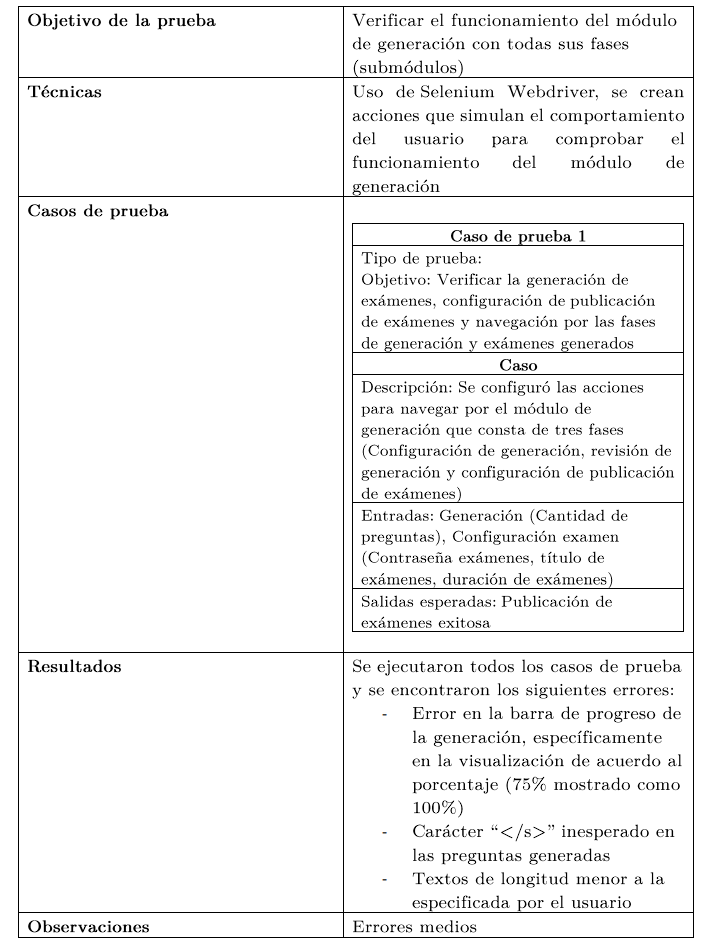
\includegraphics[width=5.7in,height=7.5in]{Chapters/06ChapterPruebas/images/caso_prueba_react_completo.png}
	    \caption{Caso de prueba inicio de sesión}
	    Fuente: Elaboración propia
        \label{tab:table1}
	\end{Center}
    \end{table}
    
    \newpage
    \begin{justify}
    En la implementación de los casos de prueba se escribieron funciones asíncronas en Javascript en los archivos correspondientes teniendo en cuenta los módulos de cada caso.
    \end{justify}
    
    \begin{justify}
    De la misma manera se realizaron el resto de casos de prueba con Selenium WebDriver, los casos de prueba completos se encuentran en los anexos.
    \end{justify}
\end{document}